\documentclass[b5paper]{book}
\usepackage[spanish]{babel}
\usepackage[latin1]{inputenc}
\usepackage{graphicx}
\special{pdf: pagesize width 17.6cm height 25.1cm}


\usepackage{fancyhdr}
\pagestyle{fancy}
\lfoot[\fancyplain{}{\thepage}]     {\fancyplain{}{}}
\cfoot[\fancyplain{}{}]     {\fancyplain{}{}}
\rfoot[\fancyplain{}{}]     {\fancyplain{}{\thepage}}


\title{PFC:An�lisis}
\author{Javier Casas Velasco}
\date{No terminado}


%\voffset=-1.54cm


\evensidemargin=-0.54cm
\oddsidemargin=-1.04cm
\textwidth=14.1cm
\headwidth=14.1cm
%\usepackage[pdftex,
%        colorlinks=true,
%        urlcolor=rltblue,       % \href{...}{...} external (URL)
%        filecolor=rltgreen,     % \href{...} local file
%        linkcolor=rltred,       % \ref{...} and \pageref{...}
%        pdftitle={Untitled},
%        pdfauthor={Your Name},
%        pdfsubject={Just a test},
%        pdfkeywords={test, testing, testable stuff},
%        pdfproducer={pdfLaTeX},
%        pdfadjustspacing=1,
%        pagebackref,
%        pdfpagemode=None,
%        bookmarksopen=true]{hyperref}
%\usepackage{color}
%\definecolor{rltred}{rgb}{0.75,0,0}
%\definecolor{rltgreen}{rgb}{0,0.5,0}
%\definecolor{rltblue}{rgb}{0,0,0.75}


\begin{document}
%\maketitle
\chapter{Introducci�n}
Hasta ahora se ha especificado en general c�mo debe ser la forma y el comportamiento de las clases y del sistema. En este punto se discutir� al detalle c�mo debe ser implementado el sistema. Por ello, hasta este punto se ha estado hablando en t�rminos abstractos, en el c�mo deber�a funcionar. En este punto se especificar�n los mecanismos y detalles concretos que llevar� la implementaci�n.

\section{Restricciones y conversiones}
Para implementar este proyecto se utilizar� el lenguaje OCaML, que al igual que cualquier otro lenguaje de programaci�n tiene sus particularidades. Por ello, a continuaci�n se especifica una peque�a gu�a para transformar los modelos de an�lisis y dise�o a este lenguaje.

\begin{itemize}
\item \textbf{Tipos de dato}
	\begin{itemize}
	\item Void o vac�o, el tipo de dato que especifica que no se pasa nada de par�metro o no se devuelve nada, pasa a llamarse \emph{unit}.
	\item Conjunto ordenado, el tipo de dato que especifica una relaci�n con varias unidades siguiendo un determinado orden, pasa a ser \emph{array} o \emph{list}, dependiendo si es necesario el acceso r�pido a un elemento concreto o la capacidad de recorrer todos los elementos en orden.
	\item Conjunto, el tipo de dato que especifica una relaci�n con varias unidades, pasa a llamarse \emph{list}, por la facilidad de a�adir o filtrar elementos.
	\item Vector, Vector4, Vector3 y Vector2 son la misma clase con distintos nombres. La �nica diferencia reside en que si a Vector4, Vector3 o Vector2 se le pasa una cantidad de par�metros distinto al n�mero de la clase, se quejan y fallan con una excepci�n. Esto se hace con el fin de favorecer los controles de precondici�n y postcondici�n.
	\end{itemize}
\item \textbf{Operaciones del lenguaje}
	\begin{itemize}
	\item OCaML es un lenguaje fuertemente tipado, con inferencia de tipos. Debido a estas caracter�sticas, no es posible hacer \emph{downcasting}, es decir, transformar una referencia a una clase en una referencia a una de sus subclases. Esto se considera una operaci�n peligrosa y ambigua, y esa es la raz�n de que el lenguaje se niegue a implementarla.
	\item Debido a que el \emph{downcasting} es imposible, el \emph{upcasting} es una operaci�n de una s�la direcci�n, y no se puede invertir. Hay que crear caminos alternativos donde el \emph{downcasting} ser�a necesario.
	\item OCaML pone muchas trabas a la hora de crear dependencias circulares. Esto ha favorecido la creaci�n de un modelo de an�lisis y dise�o libre de dependencias circulares.
	\end{itemize}
\end{itemize}

\input{diseno/arquitectura/arquitectura_actual/arquitectura_actual.tex}
\chapter{Arquitectura propuesta}
\section{Visi�n global}
El sistema pretende ser un framework para desarrollar aplicaciones interactivas. Por ello se propone l�gicamente como patr�n arquitect�nico base el MVC: Modelo-Vista-Controlador. El MVC se compone de tres subsistemas b�sicos:

\begin{figure}[]
\centering
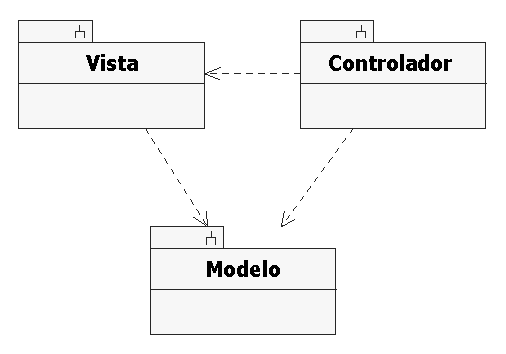
\includegraphics[width=14cm]{diseno/arquitectura/arquitectura_propuesta/diagramas/mvc.eps}
\caption{Patr�n arquitect�nico Modelo-Vista-Controlador}
\end{figure}

\begin{itemize}
\item \textbf{Modelo}
	\begin{itemize}
	\item Contiene la representaci�n y la l�gica de la aplicaci�n.
	\item Se encarga de almacenar y procesar la informaci�n.
	\end{itemize}
\item \textbf{Vista}
	\begin{itemize}
	\item Contiene los mecanismos para mostrar la informaci�n al usuario.
	\item Se encarga de mostrar la informaci�n al usuario de la aplicaci�n.
	\item Depende de Modelo.
	\end{itemize}
\item \textbf{Controlador}
	\begin{itemize}
	\item Contiene los mecanismos para recibir las peticiones del usuario.
	\item Se encarga de atender las peticiones del usuario y entregar dichas peticiones al Modelo o a la Vista.
	\item Depende de Modelo y Vista.
	\end{itemize}
\end{itemize}

El comportamiento t�pico del patr�n MVC suele ser el siguiente:
\begin{enumerate}
\item El usuario utiliza el interfaz del programa para hacer una petici�n al sistema.
\item El Controlador recibe la petici�n.
\item El Controlador env�a al Modelo una o varias peticiones de operaci�n.
\item El Modelo modifica su estado seg�n las peticiones.
\item El Controlador env�a a la Vista una petici�n de actualizaci�n.
\item La Vista recoge la informaci�n necesaria del Modelo.
\item La Vista muestra la informaci�n recogida en el interfaz del programa.
\item El usuario ve el resultado de la operaci�n en el interfaz del programa.
\end{enumerate}

\begin{figure}[]
\centering
\includegraphics[width=14cm]{diseno/arquitectura/arquitectura_propuesta/diagramas/mvc_secuencia.eps}
\caption{Modelo din�mico del patr�n arquitect�nico Modelo-Vista-Controlador}
\end{figure}

Para un videojuego, se necesita que el interfaz del programa se actualice continuamente. Por ello, en este caso el sistema se actualizar� incluso \emph{cuando el jugador no haga nada}, ya que puede que est� esperando a que ocurra alg�n evento del juego. Por ello, la asignaci�n final de responsabilidades del controlador var�a ligeramente. La \emph{no-actuaci�n} del jugador se interpretar� como una forma especial de petici�n.


\section{Dise�o de la arquitectura}
\subsection{Descomposici�n en subsistemas}
Debido a la amplitud del sistema, �ste ha sido descompuesto en un importante n�mero de subsistemas. A continuaci�n se describir�n �stos.

\begin{figure}[]
\centering
\includegraphics[width=14cm]{diseno/arquitectura/arquitectura_propuesta/diagramas/arq_detallada.eps}
\caption{Modelo arquitect�nico detallado}
\end{figure}

\subsubsection{Descomposici�n de Modelo}
Modelo se ha descompuesto en gran cantidad de subsistemas, siguiendo un modelo de \emph{grandes bloques}.
\begin{itemize}
\item \textbf{Motor gr�fico}
	\begin{itemize}
	\item Contiene los modelos de representaci�n gr�fica.
	\item Se encarga de gestionar todo lo que se muestra en pantalla. Esto incluye desde p�xeles sueltos y pol�gonos hasta pantallas o ventanas de aplicaci�n.
	\end{itemize}
\item \textbf{Motor de sonido}
	\begin{itemize}
	\item Contiene los modelos de representaci�n de sonido.
	\item Se encarga de gestionar todo lo que suena por los altavoces o auriculares.
	\end{itemize}
\item \textbf{Motor de procesos}
	\begin{itemize}
	\item Proporciona una base para la implementaci�n de la l�gica del juego.
	\item Se encarga de gestionar la l�gica del juego y de inicializar el juego una vez todos los subsistemas han sido inicializados.
	\end{itemize}
\item \textbf{Bind}
	\begin{itemize}
	\item Proporciona a la l�gica del juego un enlace con las peticiones del jugador.
	\item Se encarga de entregar las �rdenes del jugador a la l�gica del juego.
	\end{itemize}
\item \textbf{L�gica del juego}
	\begin{itemize}
	\item Este subsistema lo debe \emph{rellenar} el desarrollador que utilice el sistema para desarrollar su juego.
	\item Se encarga de procesar el modelo de comportamiento del juego, a partir de la entrada recibida a trav�s de Bind, bas�ndose en el modelo de Procesos y entregando el resultado al Motor de Sonido y al Motor Gr�fico.
	\item Depende de Motor gr�fico, Motor de sonido, Motor de procesos y Bind.
	\end{itemize}
\end{itemize}

\subsubsection{Descomposici�n de Motor gr�fico}
El motor gr�fico es un subsistema complejo, con una gran cantidad de operaciones que tratan desde el control de un p�xel hasta el control de toda la pantalla. Por ello se ha optado en descomponerlo en subsistemas. En este caso se ha utilizado un patr�n Capas. Para la implementaci�n final del mecanismo se ha optado por un patr�n estrategia aplicado a subsistemas. A continuaci�n se describir� cada uno de los subsistemas.

\begin{figure}[]
\centering
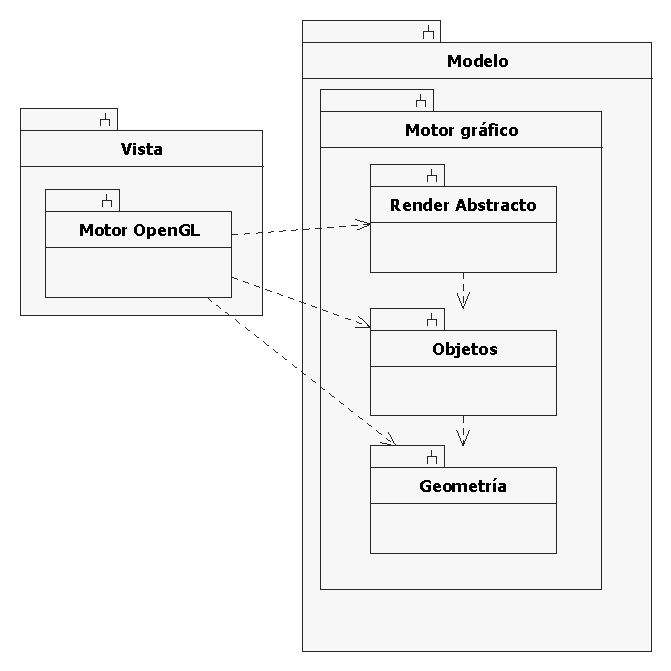
\includegraphics[width=14cm]{diseno/arquitectura/arquitectura_propuesta/diagramas/motor_grafico.eps}
\caption{Diagrama de subsistemas del Motor gr�fico}
\end{figure}

\begin{itemize}
\item \textbf{Geometr�a}
	\begin{itemize}
	\item Se encarga de almacenar y procesar los pol�gonos como unidades individuales.
	\end{itemize}
\item \textbf{Objetos}
	\begin{itemize}
	\item Proporciona un mecanismo para utilizar de una manera l�gica las mallas de pol�gonos.
	\item Se encarga de procesar las mallas como si fueran objetos f�sicos que pudieramos mover con facilidad.
	\item Se encarga de mantener la estructura general de la escena.
	\end{itemize}
\item \textbf{Render abstracto}
	\begin{itemize}
	\item Proporciona mecanismos para manipular la pantalla y c�mo se pintan las escenas.
	\item Se encarga de controlar el uso de la pantalla y los mecanismos para pintar las escenas adecuadamente.
	\end{itemize}
\item \textbf{Motor OpenGL}
	\begin{itemize}
	\item Implementa el motor gr�fico a trav�s de la biblioteca gr�fica OpenGL.
	\item Se encarga de convertir la escena abstracta que haya sido construida utilizando los subsistemas de Geometr�a, Objetos y Render Abstracto en una serie optimizada de llamadas a la biblioteca OpenGL.
	\end{itemize}
\end{itemize}

\subsection{Topolog�a del sistema}
\subsection{Descripci�n de las interfaces}

\subsection{Gesti�n de la persistencia}
Debido al tipo de sistema que se propone, es necesario proveer una estructura b�sica de preparaci�n y recuperaci�n de la informaci�n. Para ello se propone dividir este proceso en dos secciones:
\subsubsection{Preparaci�n y almacenamiento de la informaci�n}
Por una parte es necesario pre-procesar y almacenar los datos necesarios.
\begin{itemize}
\item \textbf{Mallas 3D}
	\begin{itemize}
	\item Las mallas de pol�gonos se crear�n y editar�n con la herramienta Blender.
	\item Una vez completadas las mallas de pol�gonos, se utilizar� dentro de Blender un script que generar� un archivo f�cilmente importable por el sistema.
	\end{itemize}
\item \textbf{Texturas}
	\begin{itemize}
	\item Las texturas para las mallas se generar�n con un programa de retoque fotogr�fico. Se propone por ejemplo The Gimp.
	\item Dichas texturas ser�n exportadas en formatos concretos y con caracter�sticas concretas, para que el sistema pueda importarlas.
	\end{itemize}
\item \textbf{Sonidos}
	\begin{itemize}
	\item Los sonidos ser�n preparados con un programa de edici�n de sonidos. Se propone por ejemplo el programa Audacity.
	\item Dichos sonidos ser�n exportados en formatos concretos para que el sistema pueda importarlos.
	\end{itemize}
\item \textbf{M�sica} \newline
La m�sica es m�s dif�cil de generar que los sonidos. Hay algunos tipos de programa preparados con el fin de crear m�sica. Por ello se propone que la m�sica se prepare en dos pasos
	\begin{itemize}
	\item Se genera con alg�n tipo de programa de creaci�n de m�sica, como puede ser un tracker. Para ello se propone como tracker, el ModPlug Tracker.
	\item La m�sica ser� editada y exportada a un formato de compresi�n con p�rdida de informaci�n, con el fin de evitar generar ficheros demasiado grandes. Para ello se propone el mismo programa que se utiliz� en la fase anterior: Audacity.
	\item El sistema utilizar� un mecanismo especial para importar estos ficheros, evitando cargarlos por completo, ya que pueden ser ficheros grandes.
	\end{itemize}
\end{itemize}

\subsubsection{Recuperaci�n de la informaci�n}
En este sistema se sientan las bases para crear un videojuego, pero no se especifica dicho videojuego. Por ello se debe crear un sistema muy flexible de carga de informaci�n, para que el desarrollador siga manteniendo el control sobre qu� se carga y en qu� momento. 

Por eso se propone un patr�n de f�bricas que lean ficheros e instancien las clases con la informaci�n, siempre a petici�n de los subsistemas del desarrollador.

\subsection{Aspectos globales y de seguridad}
\subsection{Aspectos de rendimiento y tama�o}




\chapter{Introducci�n}
Hasta ahora se ha especificado en general c�mo debe ser la forma y el comportamiento de las clases y del sistema. En este punto se discutir� al detalle c�mo debe ser implementado el sistema. Por ello, hasta este punto se ha estado hablando en t�rminos abstractos, en el c�mo deber�a funcionar. En este punto se especificar�n los mecanismos y detalles concretos que llevar� la implementaci�n.

\section{Restricciones y conversiones}
Para implementar este proyecto se utilizar� el lenguaje OCaML, que al igual que cualquier otro lenguaje de programaci�n tiene sus particularidades. Por ello, a continuaci�n se especifica una peque�a gu�a para transformar los modelos de an�lisis y dise�o a este lenguaje.

\begin{itemize}
\item \textbf{Tipos de dato}
	\begin{itemize}
	\item Void o vac�o, el tipo de dato que especifica que no se pasa nada de par�metro o no se devuelve nada, pasa a llamarse \emph{unit}.
	\item Conjunto ordenado, el tipo de dato que especifica una relaci�n con varias unidades siguiendo un determinado orden, pasa a ser \emph{array} o \emph{list}, dependiendo si es necesario el acceso r�pido a un elemento concreto o la capacidad de recorrer todos los elementos en orden.
	\item Conjunto, el tipo de dato que especifica una relaci�n con varias unidades, pasa a llamarse \emph{list}, por la facilidad de a�adir o filtrar elementos.
	\item Vector, Vector4, Vector3 y Vector2 son la misma clase con distintos nombres. La �nica diferencia reside en que si a Vector4, Vector3 o Vector2 se le pasa una cantidad de par�metros distinto al n�mero de la clase, se quejan y fallan con una excepci�n. Esto se hace con el fin de favorecer los controles de precondici�n y postcondici�n.
	\end{itemize}
\item \textbf{Operaciones del lenguaje}
	\begin{itemize}
	\item OCaML es un lenguaje fuertemente tipado, con inferencia de tipos. Debido a estas caracter�sticas, no es posible hacer \emph{downcasting}, es decir, transformar una referencia a una clase en una referencia a una de sus subclases. Esto se considera una operaci�n peligrosa y ambigua, y esa es la raz�n de que el lenguaje se niegue a implementarla.
	\item Debido a que el \emph{downcasting} es imposible, el \emph{upcasting} es una operaci�n de una s�la direcci�n, y no se puede invertir. Hay que crear caminos alternativos donde el \emph{downcasting} ser�a necesario.
	\item OCaML pone muchas trabas a la hora de crear dependencias circulares. Esto ha favorecido la creaci�n de un modelo de an�lisis y dise�o libre de dependencias circulares.
	\end{itemize}
\end{itemize}

\chapter{Dise�o detallado de las clases}

\section{Cargador\_malla\_simple}
Se encarga de cargar e instanciar Malla\_simple. Incluye un lexer y un parser que se encargan de la lectura del fichero. Tanto el lexer como el parser se har�n con herramientas ya disponibles: OcamlLex y OcamlYACC.

OcamlLex y OcamlYACC generan cada uno un m�dulo nuevo que es utilizado por Cargador\_malla\_simple. Estos m�dulos se llaman \emph{Cargador\_malla\_lexer} y \emph{Cargador\_malla\_parser}.

\begin{itemize}
\item \textbf{Relaciones:}
	\begin{itemize}
	\item <<instantiate>> Clases del tipo *\_simple. \newline
		Instancia Malla\_simple y las clases que utilice Malla\_simple. Adem�s, realiza la interconexi�n de estas clases.
	\item <<uso>> Utiliza una instancia de Dispositivo\_entrada\_caracteres para leer el fichero.
	\end{itemize}
\item \textbf{M�todos:}
	\begin{itemize}
	\item +cargar(d : Dispositivo\_entrada\_caracteres) : malla \newline
		Llama a cargar\_malla\_simple. Devuelve el resultado como malla, y no malla\_simple, con el fin de utilizarlo para alg�n tipo de cargador abstracto.
	\item +cargar\_malla\_simple(d : Dispositivo\_entrada\_caracteres) : Malla\_simple \newline
		Carga e instancia una Malla\_simple desde el dispositivo de entrada indicado.
	\end{itemize}
\end{itemize}

\subsection{El lexer}
El lexer se encarga de leer los caracteres del fichero y transformarlos en elementos de prean�lisis para el parser. A continuaci�n se describen estos elementos.

\newcommand{\elemento}[2]{\item \textbf{#1} \newline #2}
\begin{itemize}
\elemento{\emph{espacio en blanco}}{Ignorado}
\elemento{\emph{tabulador}}{Ignorado}
\elemento{\emph{retorno de carro}}{Ignorado}
\elemento{\#, \emph{cualquier caracter excepto retorno de carro}, \emph{retorno de carro}}{Ignorado, es un comentario}
\elemento{\emph{n�mero real}}{REAL}
\elemento{\emph{n�mero entero}}{ENTERO}
\elemento{", \emph{cadena de caracteres}, "}{CADENA}
\elemento{version}{VERSION}
\elemento{o}{OBJETO}
\elemento{nv}{NUMVERTICES}
\elemento{v}{VERTICE}
\elemento{nm}{NUMMATERIALES}
\elemento{m}{MATERIAL}
\elemento{tex}{TEXTURA}
\elemento{notex}{NOTEXTURA}
\elemento{esp}{ESPECULAR}
\elemento{emi}{EMISION}
\elemento{nf}{NUMCARAS}
\elemento{f}{CARA}
\elemento{fm}{MATERIAL\_CARA}
\elemento{fv}{VERTICE\_CARA}
\elemento{fvuc}{VERTICE\_CARA\_UV\_COLOR}
\elemento{\emph{fin de fichero}}{EOF}
\end{itemize}

\subsection{El parser}
El parser se encarga de procesar los elementos de prean�lisis del lexer, comprobar que siguen la sintaxis especificada y construir la malla a partir de la informaci�n del fichero. A continuaci�n se especifican las reglas del parser.

En may�sculas, los terminales definidos en la secci�n anterior. En min�sculas, los auxiliares. Cada palabra es un \emph{s�mbolo}. 

S�mbolo inicial: main\newline
\newcommand{\regla}[2]{\item\textbf{#1} -\textgreater \newline #2}
\begin{itemize}
\regla{main}{version nombre vertices materiales caras EOF}
\regla{version}{VERSION REAL}
\regla{nombre}{OBJETO CADENA}
\regla{vertices}{NUMVERTICES ENTERO desc\_vertices}
\regla{desc\_vertices}{desc\_vertice desc\_vertices \newline \textbar desc\_vertice}
\regla{desc\_vertice}{VERTICE REAL REAL REAL REAL REAL REAL}
\regla{materiales}{NUMMATERIALES ENTERO desc\_materiales}
\regla{desc\_materiales}{desc\_material desc\_materiales \newline \textbar desc\_material}
\regla{desc\_material}{MATERIAL CADENA textura difuso especular emision}
\regla{textura}{TEXTURA CADENA \newline \textbar NOTEXTURA}
\regla{difuso}{DIFUSO REAL REAL REAL REAL}
\regla{especular}{ESPECULAR REAL REAL REAL REAL REAL}
\regla{emisi�n}{EMISION REAL REAL REAL REAL}
\regla{caras}{NUMCARAS ENTERO desc\_caras}
\regla{desc\_caras}{desc\_cara desc\_caras \newline \textbar desc\_cara}
\regla{desc\_cara}{CARA material\_cara vertices\_cara}
\regla{material\_cara}{MATERIAL\_CARA ENTERO}
\regla{vertices\_cara}{vertice\_cara vertice\_cara vertice\_cara \newline \textbar vertice\_cara vertice\_cara vertice\_cara vertice\_cara}
\regla{vertice\_cara}{VERTICE\_CARA ENTERO \newline \textbar VERTICE\_CARA\_UV\_COLOR ENTERO REAL REAL REAL REAL REAL REAL}
\end{itemize}






\end{document}
